\documentclass{article}
\textheight 22.5truecm \textwidth 14.5truecm
\setlength{\oddsidemargin}{0.35in}\setlength{\evensidemargin}{0.35in}

\usepackage[utf8]{inputenc}
\usepackage[russian]{babel}
\usepackage{graphicx}
\usepackage{amsmath}
\usepackage{breqn}
\usepackage{wrapfig}
\usepackage{float}
\usepackage{multirow}
\usepackage{caption}
\usepackage{subcaption}

\graphicspath{ {./data/images} }
\author{Александр Романов Б01-110}
\date{}
\title{5.1 Измерения коэффициента ослабления потока \(\gamma\)-лучей в веществе и определение их энергии}

\begin{document}
\maketitle
\section{Введение}
\subsection{О работе}
С помощью сцинтилляционного счетчика измеряются линейные коэффициенты ослабления потока \(\gamma\)-лучей в
свинце, железе и алюминии. По их величине определяется энергия \(\gamma\)-квантов.
\subsection{Экспериментальная установка}
\begin{figure}[H]
	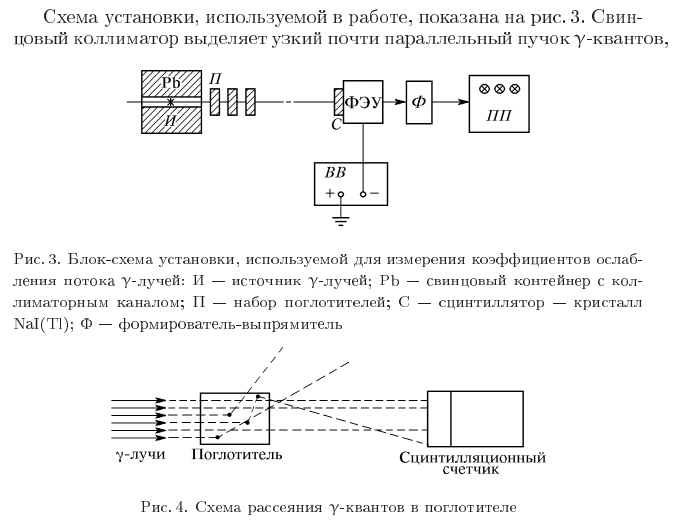
\includegraphics[width=\textwidth]{scheme.png}
\end{figure}
\section{Работа}
Включим пересчётный прибор и высоковольтный выпрямитель. Дадим им прогреться.

Измерим число частиц, попадающих в счётчик в отсутствии поглотителя. Получим \(N_0 = 168687\) частиц за
20 сек. Поставим длинный поглотитель и снова измерим. Получим \(N_0 = 2093\) за 60 сек. Последний результат
получился во много раз меньше. Т.е. установка исправна.

Будем поочереди ставить на коллиматор таблетки из разных материалов, измерять их суммарную толщину и
измерять число частиц.

\subsection{Al}

\begin{table}[H]
    \centering
    \begin{tabular}{|c|c|c|c|c|c|}
    \hline
        plates number & 1 & 2 & 3 & 4 & 5 \\ \hline
        length, mm & 20 & 40 & 60 & 80 & 100 \\ \hline
        time, s & 25 & 36 & 60 & 60 & 90 \\ \hline
        particles number & 139143 & 130440 & 145021 & 97203 & 100231 \\ \hline
				$\mu,\; mm^{-1}$ & 0.0208 & 0.0211 & 0.0208 & 0.0206 & 0.0202 \\ \hline
        relative error & 0.0027 & 0.0028 & 0.0026 & 0.0032 & 0.0032 \\ \hline
    \end{tabular}
\end{table}

Среднее значение: \(\mu_a = 0.0207 \pm 6.6e-5,\; mm^{-1}\)

\subsection{Fe}

\begin{table}[H]
    \centering
    \begin{tabular}{|c|c|c|c|c|c|}
    \hline
        plates number & 1 & 2 & 3 & 4 & 5 \\ \hline
        length, mm & 10 & 20.1 & 30.3 & 40.4 & 50.6 \\ \hline
        time, s & 20 & 36 & 60 & 110 & 150 \\ \hline
        particles number & 95194 & 93169 & 90875 & 98769 & 82301 \\ \hline
        $\mu,\; mm^{-1}$ & 0.0572 & 0.0588 & 0.0567 & 0.0554 & 0.0540 \\ \hline
        relative error & 0.0032 & 0.0033 & 0.0033 & 0.0032 & 0.0035 \\ \hline
    \end{tabular}
\end{table}

Среднее значение: \(\mu_a = 0.0564 \pm 1.9e-4,\; mm^{-1}\)

\subsection{Pb}

\begin{table}[!ht]
    \centering
    \begin{tabular}{|c|c|c|c|c|c|}
    \hline
        plates number & 1 & 2 & 3 & 4 & 5 \\ \hline
        length, mm & 5.2 & 9.9 & 14.8 & 19.6 & 23.9 \\ \hline
        time, s & 29 & 46 & 60 & 81 & 120 \\ \hline
        particles number & 128147 & 121544 & 92433 & 77973 & 83105 \\ \hline
        $\mu, mm^{-1}$ & 0.1243 & 0.1172 & 0.1149 & 0.1107 & 0.1046 \\ \hline
        relative error & 0.0028 & 0.0029 & 0.0033 & 0.0036 & 0.0035 \\ \hline
    \end{tabular}
\end{table}

Среднее значение: \(\mu_a = 0.1144 \pm 4.1e-4,\; mm^{-1}\)

\subsection{Энергия}
Определим среднюю энергию \(\gamma\)-лучей при помощи графика:

\begin{figure}[H]
	\centering
	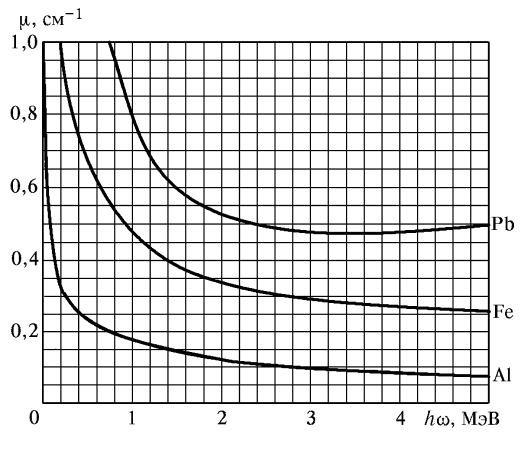
\includegraphics[width=0.6\textwidth]{plot.png}
	\caption{Полные коэффициенты ослабления потока $\gamma$-лучей в алминии, железе и свинце}
\end{figure}

Результаты:
\[ E_{Al} = 0.7\; MeV \]
\[ E_{Fe} = 0.75\; MeV \]
\[ E_{Pb} = 0.75\; MeV \]

\section{Выводы}
В ходе выполнения работы были измерены коэффициенты поглощения \(\gamma\)-лучей в различных веществах:
\[ \mu_{Al} = 0.0207 \pm 6.6e-5,\; mm^{-1} \]
\[ \mu_{Fe} = 0.0564 \pm 1.9e-4,\; mm^{-1} \]
\[ \mu_{Pb} = 0.1144 \pm 4.1e-4,\; mm^{-1} \]

Этим значениям были сопоставленны соответсвующие значения энергии \(\gamma\)-лучей из справочных материалов.
Все значения оказались близки друг к другу и составляют в среднем \(0.74 \pm 0.4\; MeV\)
\end{document}
